% http://staff.itee.uq.edu.au/janetw/cmc/chapters/BackProp/index2.html
% http://outlace.com/Beginner-Tutorial-Backpropagation/
% http://neuralnetworksanddeeplearning.com/chap2.html
% http://staff.itee.uq.edu.au/janetw/cmc/chapters/BackProp/slides/Backprop_files/frame.htm
% http://staff.itee.uq.edu.au/janetw/cmc/chapters/BackProp/
% http://home.agh.edu.pl/~vlsi/AI/backp_t_en/backprop.html
% https://www.google.cl/webhp?sourceid=chrome-instant&ion=1&espv=2&ie=UTF-8#safe=off&q=backpropagation+practice+example
% https://ayearofai.com/rohan-4-the-vanishing-gradient-problem-ec68f76ffb9b#.9ntv81akz

\ifx\du\undefined
  \newlength{\du}
\fi
\newcommand{\nweigth}[2]{$W^{#1}_{#2} - \alpha\frac{\partial J}{\partial W^{#1}_{#2}}$}
\newcommand{\w}[2]{$W^{#1}_{#2}$}

\setlength{\du}{1\unitlength}
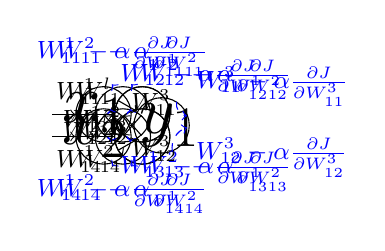
\begin{tikzpicture}[font=\small]
\tikzstyle{neuron}=[circle,draw, minimum size=2em]
\tikzstyle{update}=[dashed, blue]

\pgftransformxscale{1.000000}
\pgftransformyscale{-1.000000}

\coordinate (x1)    at (0.000000\du, 0.000000\du);
\coordinate (x2)    at (0.000000\du, 8.000000\du);

\coordinate (i)     at (3.000000\du, 0.000000\du);
\coordinate (ii)    at (3.000000\du, 8.000000\du);

\coordinate (iv)    at (10.000000\du, 0.000000\du);
\coordinate (v)     at (10.000000\du, 8.000000\du);

\coordinate (vii)   at (17.000000\du, 0.000000\du);
\coordinate (viii)  at (17.000000\du, 8.000000\du);

\coordinate (ix)   at (17.000000\du, 0.000000\du);
\coordinate (diez)  at (17.000000\du, 8.000000\du);


\coordinate (x)     at (24.000000\du, 4.000000\du);
\coordinate (y)     at (27.000000\du, 4.000000\du);


%%%%%%%%%%%%%%%%%%%%%%%%%%%%%%%%%%%%%%%%%%%%%%%%%%%%%%%%%%
% ENTRADA
\node (X1) at (x1) {\Huge $x_1$};
\node (X2) at (x2) {\Huge $x_2$};

% CAPA DE ENTRADA
\node[neuron] (A) at  (i) {}; % A
\node[neuron] (B) at  (ii)  {}; % B

% CAPA 1
\node[neuron] (C) at  (iv)  {}; % C
\node[neuron] (D) at  (v)  {}; % D

% CAPA 2
\node[neuron] (E) at  (vii)  {}; % E
\node[neuron] (F) at  (viii)  {}; % F

% CAPA 2
\node[neuron] (H) at  (ix)  {}; % E
\node[neuron] (I) at  (diez)  {}; % F

% CAPA DE SALIDA
\node[neuron] (G) at  (x)  {}; % G

% SALIDA
\node (out) at (y) {\Huge $y_1$};
%%%%%%%%%%%%%%%%%%%%%%%%%%%%%%%%%%%%%%%%%%%%%%%%%%%%%%%%%%


\draw[->] (X1) -- (A);
\draw[->] (X2) -- (B);


%%%%%%%%%%%%%%%%%%%%%%%%%%%%%%%%%%%%%%%%%%%%%%%%%%%%%%%%%%
%%%%%%%%%%%%%%%%%%%%%%%%%%%%%%%%%%%%%%%%%%%%%%%%%%%%%%%%%%
\draw[->] (A) -- node[above, pos=0.2] (W_1_11) {\w{1}{11}} (C);
\draw[->] (A) -- node[left , pos=0.2] (W_1_12) {\w{1}{12}} (D);
\draw[->] (B) -- node[left , pos=0.2] (W_1_13) {\w{1}{13}} (C);
\draw[->] (B) -- node[below, pos=0.2] (W_1_14) {\w{1}{14}} (D);

%\draw[->, dashed, blue] (C) to [bend left=40] node[above] {$W^{1}_{11} - \alpha\frac{\partial J}{\partial W^{1}_{11}}$} (W_1_11);
\draw[->, update] (C) to [bend left=40] node[above] {\nweigth{1}{11}} (W_1_11);
\draw[->, update] (D) to [bend left=50] node[above right, pos=0.98] {\nweigth{1}{12}} (W_1_12);

\draw[->, update] (C) to [bend right=50] node[below right, pos=0.98] {\nweigth{1}{13}} (W_1_13);
\draw[->, update] (D) to [bend right=40] node[below] {\nweigth{1}{14}} (W_1_14);

%%%%%%%%%%%%%%%%%%%%%%%%%%%%%%%%%%%%%%%%%%%%%%%%%%%%%%%%%%
%%%%%%%%%%%%%%%%%%%%%%%%%%%%%%%%%%%%%%%%%%%%%%%%%%%%%%%%%%
\draw[->] (C) -- node[above, pos=0.2] (W_2_11) {\w{l}{11}} (E);
\draw[->] (C) -- node[left , pos=0.2] (W_2_12) {\w{2}{12}} (F);
\draw[->] (D) -- node[left , pos=0.2] (W_2_13) {\w{2}{13}} (E);
\draw[->] (D) -- node[below, pos=0.2] (W_2_14) {\w{2}{14}} (F);

\draw[->, update] (E) to [bend left=40] node[above] {\nweigth{2}{11}} (W_2_11);
\draw[->, update] (F) to [bend left=50] node[above right, pos=0.98] {\nweigth{2}{12}} (W_2_12);

\draw[->, update] (E) to [bend right=50] node[below right, pos=0.98] {\nweigth{2}{13}} (W_2_13);
\draw[->, update] (F) to [bend right=40] node[below] {\nweigth{2}{14}} (W_2_14);

%%%%%%%%%%%%%%%%%%%%%%%%%%%%%%%%%%%%%%%%%%%%%%%%%%%%%%%%%%
%%%%%%%%%%%%%%%%%%%%%%%%%%%%%%%%%%%%%%%%%%%%%%%%%%%%%%%%%%
\draw[->] (E) -- node[right, pos=0.2] (W_3_11) {\w{3}{11}} (G);
\draw[->] (F) -- node[right, pos=0.2] (W_3_12) {\w{3}{12}} (G);

\draw[->, update] (G) to [bend  left=50] node[above right, pos=0.98] {\nweigth{3}{11}} (W_3_11);
\draw[->, update] (G) to [bend right=40] node[below right, pos=0.98] {\nweigth{3}{12}} (W_3_12);


\draw[->] (G) -- (out);
\end{tikzpicture}
